\documentclass[xcolor=dvipsnames]{beamer} 
\usecolortheme[named=Gray]{structure} 
\setbeamertemplate{blocks}[shadow=true] 
\usepackage{ucs}
\usepackage{wasysym}
\usepackage[utf8x]{inputenc}
%\input beamerthemeumbc4.sty
%\usepackage{beamerthemeumbc4}
\useoutertheme{shadow}
%\usetheme{Madrid} % My favorite!
%\usetheme{Boadilla} % Pretty neat, soft color.
%\usetheme{umbc4}
\usetheme{Ilmenau}
%\usetheme{Amsterdam}
%\usetheme{CambridgeUS}
%\usetheme{Berlin}
%\usetheme{Warsaw}
%\usetheme{Bergen} % This template has nagivation on the left
%\usetheme{Frankfurt} % Similar to the default 
%with an extra region at the top.
%\usetheme{Darmstadt} % not so good
\usecolortheme{beaver} % Simple and clean template
% Uncomment the following line if you want %
% page numbers and using Warsaw theme%
% \setbeamertemplate{footline}[page number]
%\setbeamercovered{transparent}
\setbeamercovered{invisible}
% Get rid of navigation
\setbeamertemplate{navigation symbols}{} 
% To remove the navigation symbols from 
% the bottom of slides%
\setbeamertemplate{navigation symbols}{} 
%
\usepackage{graphicx}
%\usepackage{bm}         % For typesetting bold math (not \mathbold)
%\logo{\includegraphics[height=0.6cm]{debian-text.eps}}
%
\title[Un proiect universal, cu o comunitate globală]{Proiectul Debian}
\author{Victor Ni\c{t}u}
\institute[Ceata, Debian România]
{
Fundația Ceata\\Comunitatea Debian din Rom\^{a}nia\\
\medskip
{\emph{victor@debian-linux.ro}}
}
\date{11 iunie 2012\\București, România}
% \today will show current date. 
% Alternatively, you can specify a date.
%
\begin{document}
%
\begin{frame}
\titlepage
\end{frame}
%
\begin{frame}
\frametitle{Sumar}
\begin{itemize}
\item Introducere în filosofia Debian
\item Concepte specifice
\item Statistici
\item Comunitatea globală
\item Comunitatea din România
\item Cum devin membru? De ce?
\end{itemize}
\end{frame}
%
\section{Filosofia Debian}
\begin{frame}
\frametitle{Concepte specifice Debian}
\begin{block}{}
\begin{itemize}
\item Nu este deținut de o companie
\item Asigură libertatea ideilor și programelor componente
\item Este cel mai mare proiect al unei comunități libere
\item Universal - rulează pe o multitudine de platforme
\item Accesibil - optimizat pentru utilizatori cu deficiențe
\end{itemize}
\end{block}
\end{frame}

\subsection{Documentele libertății}
\begin{frame}
\frametitle{Debian înseamnă libertate}
\footnotesize{
\begin{thebibliography}{99}
 \bibitem[Label1]{key1} Contractul Social Debian
 \newblock Documentul esențial în relația Debian - dezvoltatori/utilizatori
 \newblock \emph{Garantează libertatea proiectului, precum și persistența acesteia.}
 \bibitem[Label2]{key2} DFSG
 \newblock Indicațiile Debian în privința programelor libere \\
 (en. Debian Free Software Guidelines)
 \newblock \emph{Extinde Contractul Social printr-un set de reguli ce concretizează definiția programelor libere.}
\end{thebibliography}
}
\end{frame}
%

\begin{frame}
\frametitle{Debian \^{i}nseamnă libertate}
\begin{block}
{Indicații extrase din DFSG}
Caracteristici ale unui program liber:\\
\begin{itemize}
\item poate fi redistribuit gratuit
\item include codul sursă
\item permite modificarea / derivarea lui
\item elimină orice discriminare față de persoane / grupuri / intenții
\item asigură păstrarea licenței
\item licența nu trebuie să fie valabilă doar în cadrul Debian
\end{itemize}
\end{block}
\begin{normalsize}
\hfill Licențe acceptate ca libere: GPL, BSD, CC-BY-SA
\end{normalsize}
\end{frame}
%
\subsection{Dezvoltare în interesul public}
\begin{frame}
\frametitle{Structura proiectului}
\begin{block}
{}
Debian este marcă înregistrată a SPI (Software in Public Interest)
\end{block}
\begin{block}{}
Ierarhia și structura decizională este alcătuită exclusiv din membrii proiectului
\end{block}
\begin{block}{}
Există un lider de proiect, votat anual de către membri, care reprezintă interesele Debian în mod public
\end{block}
\begin{normalsize}\hfill
Orice membru Debian poate interveni în direcția care prezintă interes pentru el, iar decizia se va lua de comun acord.
\end{normalsize}
  \raisebox{40mm}[0pt][0pt]{%
    \begin{pgfpicture}{-7mm}{30mm}{0mm}{0mm}
		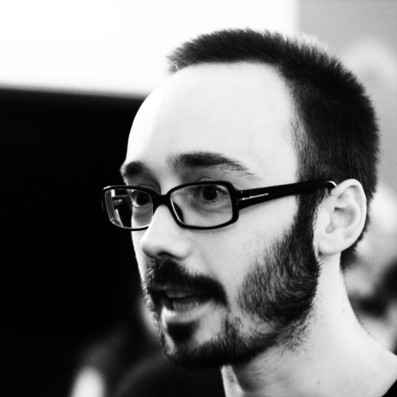
\includegraphics[height=1.75cm]{../images/zack.jpg}
    \end{pgfpicture}
  }
\end{frame}
%
\subsection{Sistemul de operare universal}
\begin{frame}
\frametitle{Disponibilitate și accesibilitate}
\begin{block}
{Hardware}
Pentru a rula sistemul de operare, este necesar un minim de hardware disponibil.
\end{block}
\begin{block}
{Arhitecturi}
Debian poate fi instalat atât pe calculatorul personal, cât și pe dispozitive minimaliste, telefoane mobile sau servere.
\end{block}
\begin{block}
{Portare}
Debian nu este construit doar în jurul nucleului Linux. Astăzi există portări ale sistemului de operare și către nucleele Hurd și kFreeBSD.
\end{block}
\end{frame}
%
\begin{frame}
\frametitle{Disponibilitate și accesibilitate}
\begin{block}
{Accesibil}
Debian este configurat din start pentru a putea fi utilizat de oricine.\\
\begin{itemize}
\item Suport nativ pentru terminale Braille
\item Integrare implicită a sintezei vocale
\item Optimizări ușoare ale consolei pentru acomodare la diverse condiții de accesibilitate (mai mare, mai contrastat etc.)
\item Detectare implicită a dispozitivelor auxiliare, încă de la pornirea programului de instalare
\item Este tradus în peste 50 de limbi
\end{itemize}
\end{block}
\end{frame}

\section{Statistici}
\subsection{Debian pe hartă}
\begin{frame}
\frametitle{Debian în cifre}
\begin{block}
{Dezvoltatori pe regiuni geografice}
\begin{itemize}
\item Finlanda este pe primul loc, procentual, cu \textbf{21} de dezvoltatori activi și o proporție de 4 / milion de locuitori
\item \textbf{SUA}, \textbf{Germania} și \textbf{Franța} sunt primele ca număr total de dezvoltatori Debian, cu \textbf{165}, \textbf{155}, respectiv \textbf{94} de conturi active.
\item România este pe poziția \textbf{46}, cu 2 membri, și unul singur activ.
\end{itemize}
\end{block}
\begin{block}
{Generalizări}
În total, membri din \textbf{59} de țări sunt implicați direct în dezvoltare.\\
Un număr de \textbf{920}, dintr-un total de \textbf{1490}, sunt activi și au adus contribuții importante proiectului.
\end{block}
\end{frame}

\subsection{Debian în relație cu alte distribuții}
\begin{frame}
\frametitle{Debian și aplicațiile server}
  \raisebox{-40mm}[0pt][0pt]{%
    \begin{pgfpicture}{-10mm}{-2.5mm}{0mm}{0mm}
		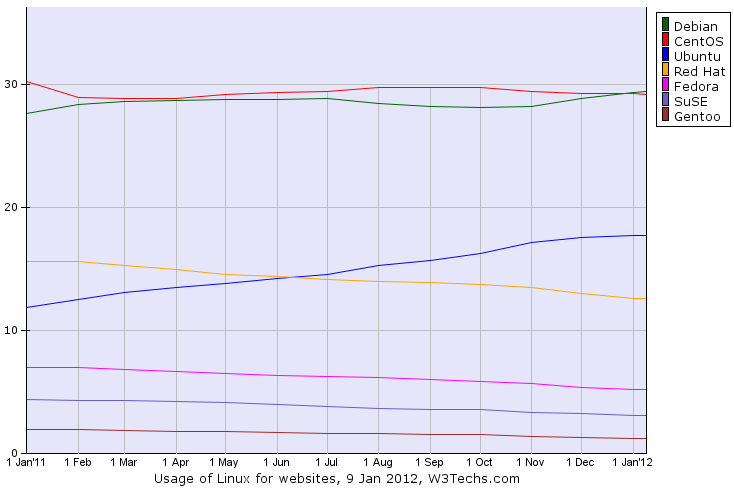
\includegraphics[height=6cm]{../images/debian-server.png}
    \end{pgfpicture}
  }
\end{frame}

\begin{frame}
\frametitle{Debian - arborele genealogic}
  \raisebox{-40mm}[0pt][0pt]{%
    \begin{pgfpicture}{-65mm}{8mm}{0mm}{0mm}
		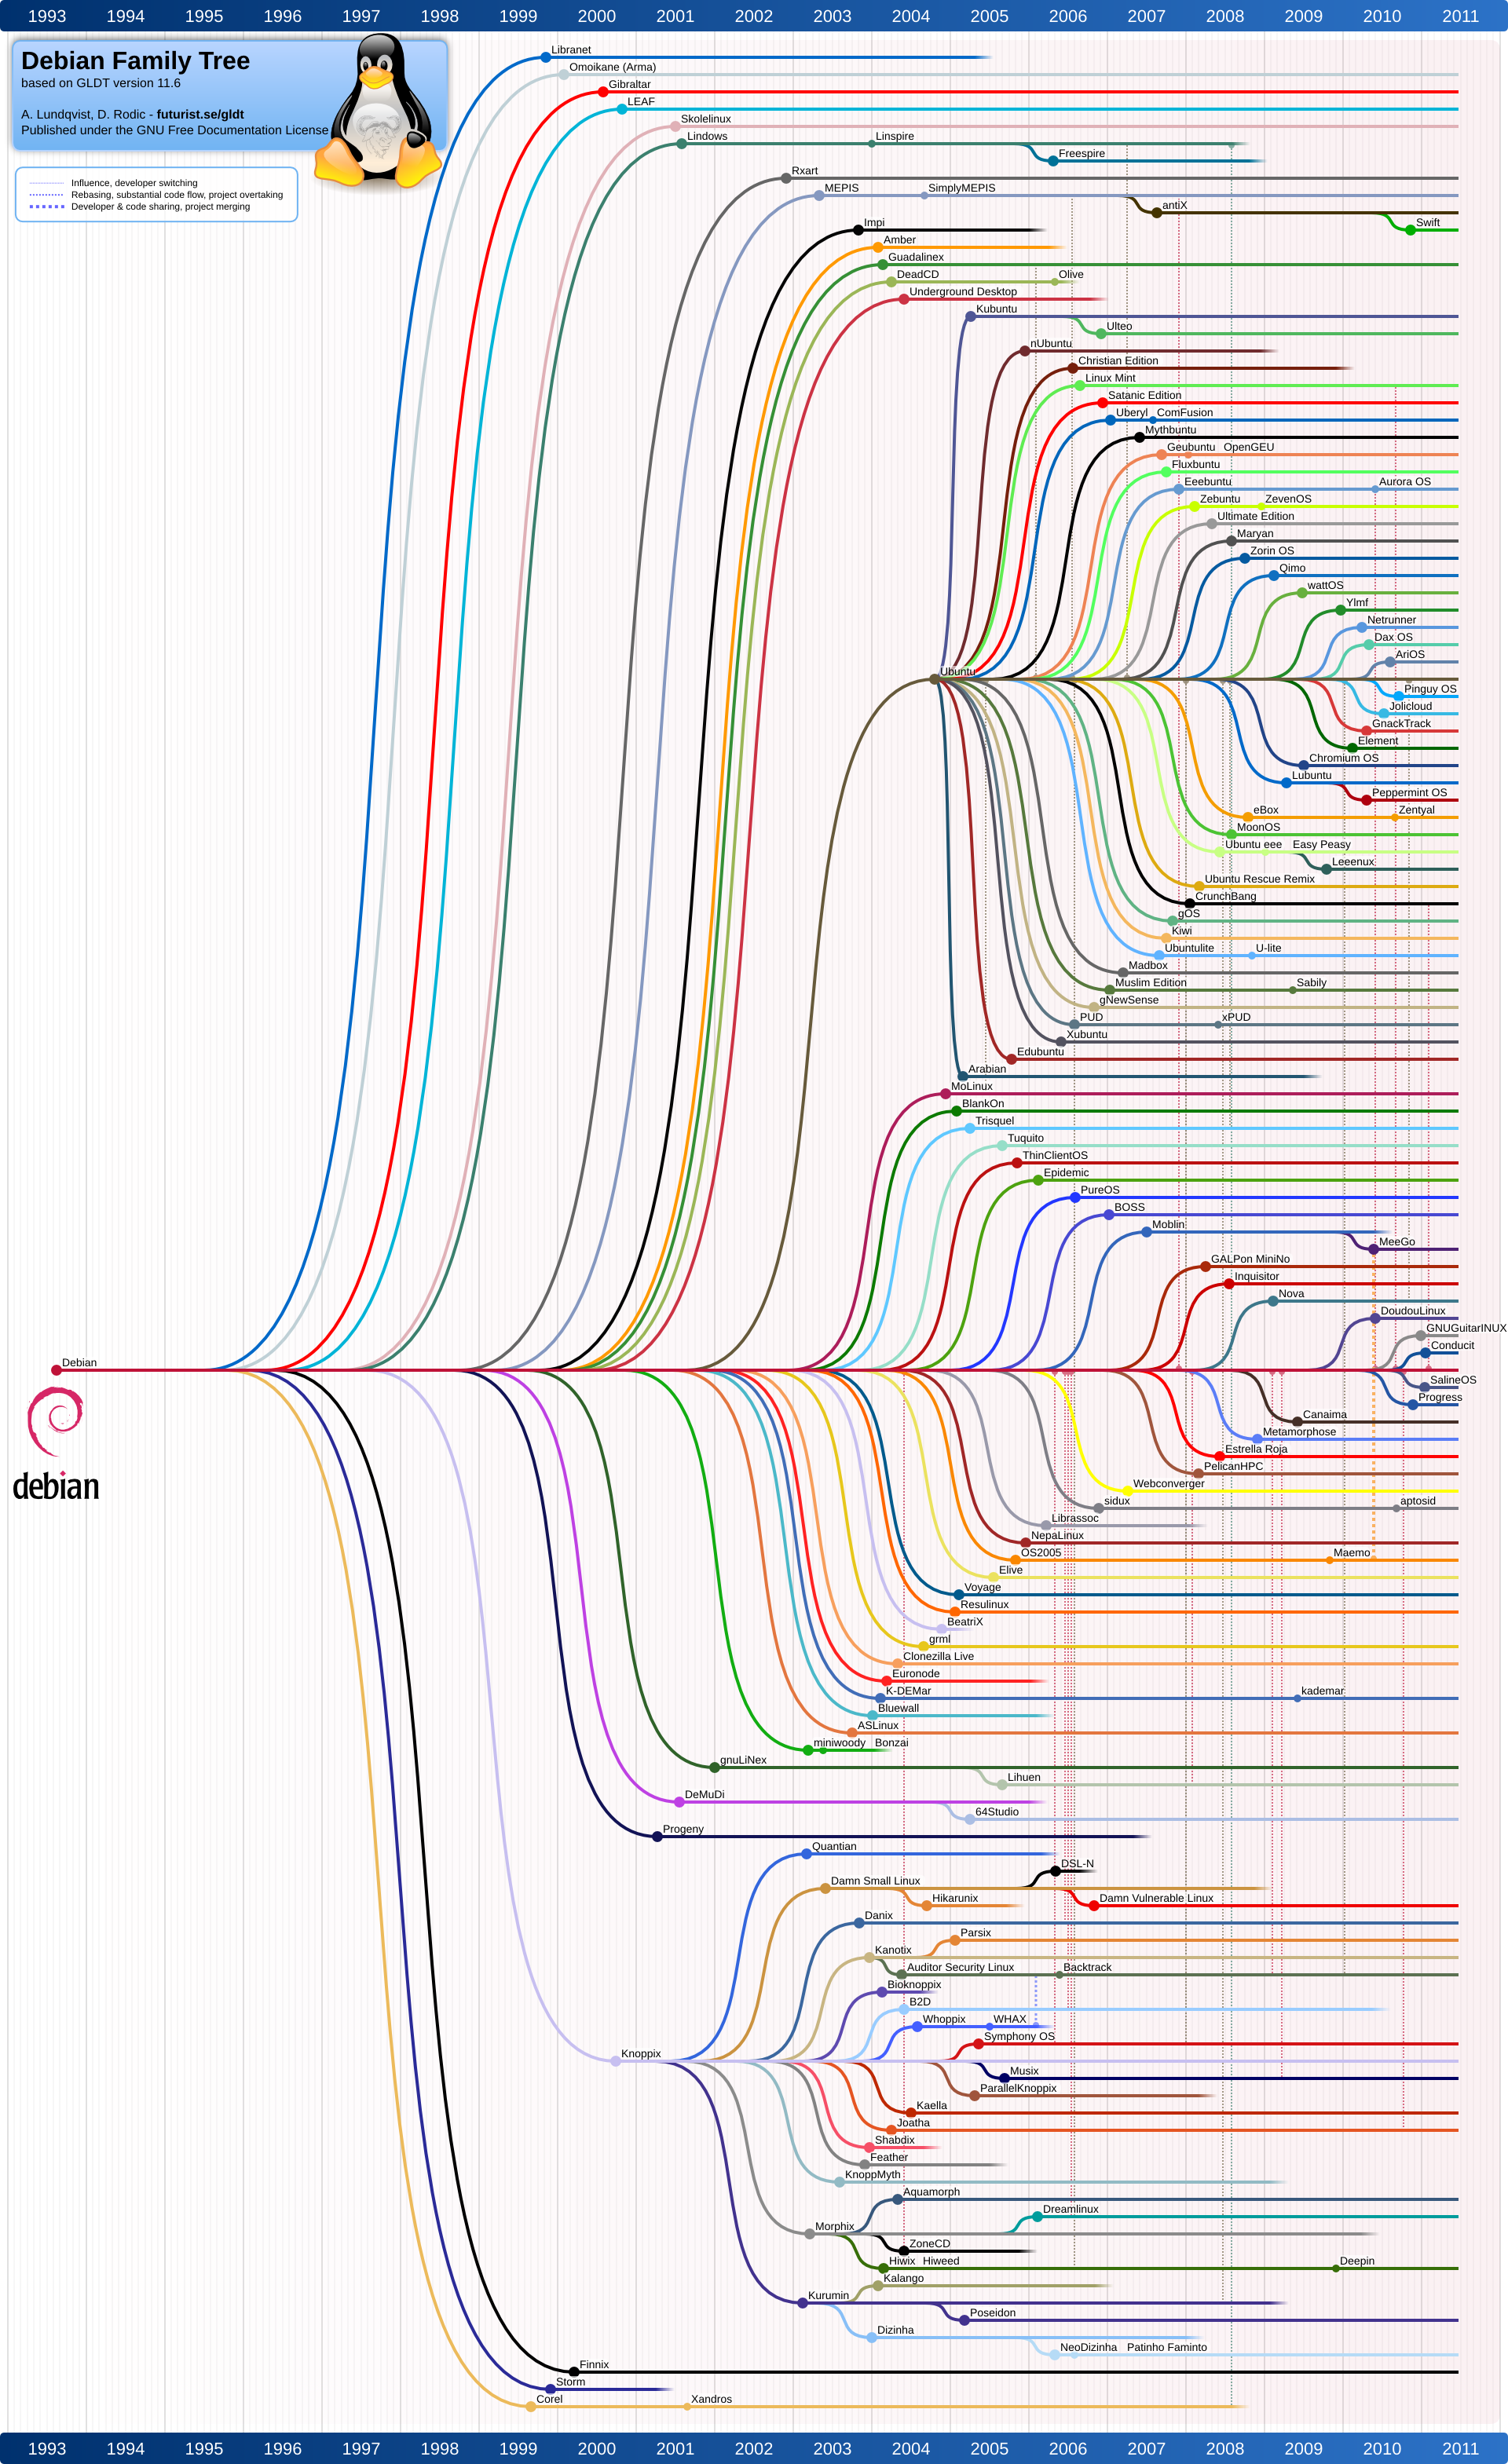
\includegraphics[height=6.5cm]{../images/debian-tree.png}
    \end{pgfpicture}
  }
	\begin{itemize}
		\item Ubuntu
		\item Linux Mint
		\item MeeGo
		\item Knoppix
		\item DSL (Damn Small Linux)
	\end{itemize}
\end{frame}

\section{Noutăți}
\begin{frame}
\frametitle{Debian 7.0 - Wheezy?}
\begin{block}
{Când?}
\begin{small}
Spre sfârșitul lui iunie 2012, Debian/testing va intra în perioada de \emph{freeze}, și se va lucra exclusiv la repararea defectelor ce previn lansarea.\\
Ne așteptăm ca în prima jumătate a lui 2013 noua versiune să fie în curs de lansare.
\end{small}
\end{block}
\end{frame}

\begin{frame}
\frametitle{Freeze}
  \raisebox{-40mm}[0pt][0pt]{%
    \begin{pgfpicture}{-12.5mm}{0mm}{0mm}{0mm}
		
\includegraphics[height=7cm]{../images/freeze.png}
    \end{pgfpicture}
  }
\end{frame}

\subsection{Noutăți în Wheezy}
\begin{frame}
\frametitle{Ce e nou?}
\begin{block}
{Multi-arch}
Posibilitatea de a crea pachete pentru diferite arhitecturi fără necesitatea instalării acestora (dpkg/multiarch).
\end{block}
\begin{block}
{Instalare mai accesibilă}
Suport implicit pentru autentificare WPA\\
Suport pentru ARM
\end{block}
\begin{block}
{Actualizarea nucleului}
Debian GNU/Linux va rula pe un nucleu din generația 3.x.
\end{block}
\end{frame}


\section{Comunitatea Debian}
\begin{frame}
\frametitle{Planeta Debian}
\begin{block}
{Ce este? Ce are special?}
\begin{itemize}
\item Oameni implicați într-o gamă largă de domenii
\item Oameni care se întâlnesc rar, și cu multă plăcere!
\item Activiști în favoarea libertății informatice și de exprimare
\item Jurnalișți, ingineri, utilizatori pasionați, hackeri sau artiști, toți lucrează pe același front
\end{itemize}
  \raisebox{0mm}[0mm][0pt]{%
    \begin{pgfpicture}{-50mm}{10mm}{0mm}{0mm}
		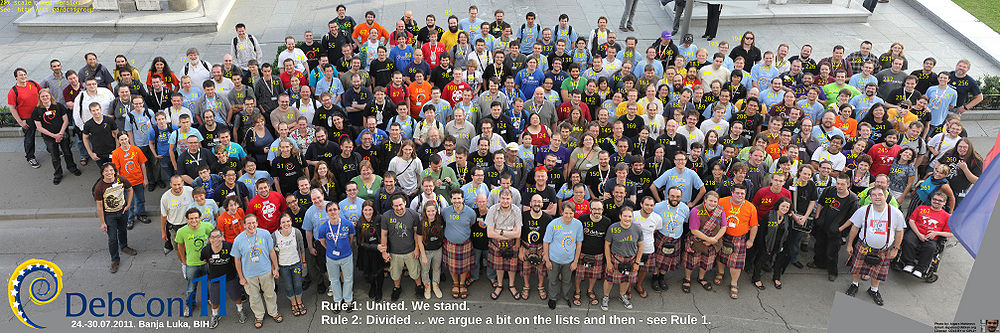
\includegraphics[height=2cm]{../images/debconf11.jpg}
    \end{pgfpicture}
  }
\end{block}
\end{frame}

\subsection{De ce să mă implic?}
\begin{frame}
\frametitle{De ce? Cum? Eu?}
\begin{block}
{Părțile bune}
\begin{itemize}
\item Poți influența direct cursul proiectului
\item Ocazia de a lucra cu persoane remarcabile în domeniu
\item Indiferent ce știi să faci, poate fi utilizat productiv
\item Recunoașterea imediată și obiectivă a realizărilor
\item Mediu foarte prietenos
\end{itemize}
\end{block}
\begin{block}
{Părțile rele}
\begin{itemize}
\item Deciziile bune se iau greu
\item Responsabilitatea crește cu numărul distribuțiilor derivate
\item Dispersarea pe glob face sincronizările online foarte dificile
\end{itemize}
\end{block}
\end{frame}

\subsection{Comunitatea Debian din România}
\begin{frame}
\frametitle{Povestea debian-linux.ro}
\begin{block}{}
...a început in februarie 2011, cu ajutorul ServerHost.\\
\hfill\\
Ce am construit noi între timp:
\begin{itemize}
\item Un forum cu activitate moderată
\item Un sit informativ despre Debian
\item Bazele unei comunități unite
\end{itemize}
\end{block}
  \raisebox{0mm}[0mm][0pt]{%
    \begin{pgfpicture}{-75mm}{-8mm}{0mm}{0mm}
		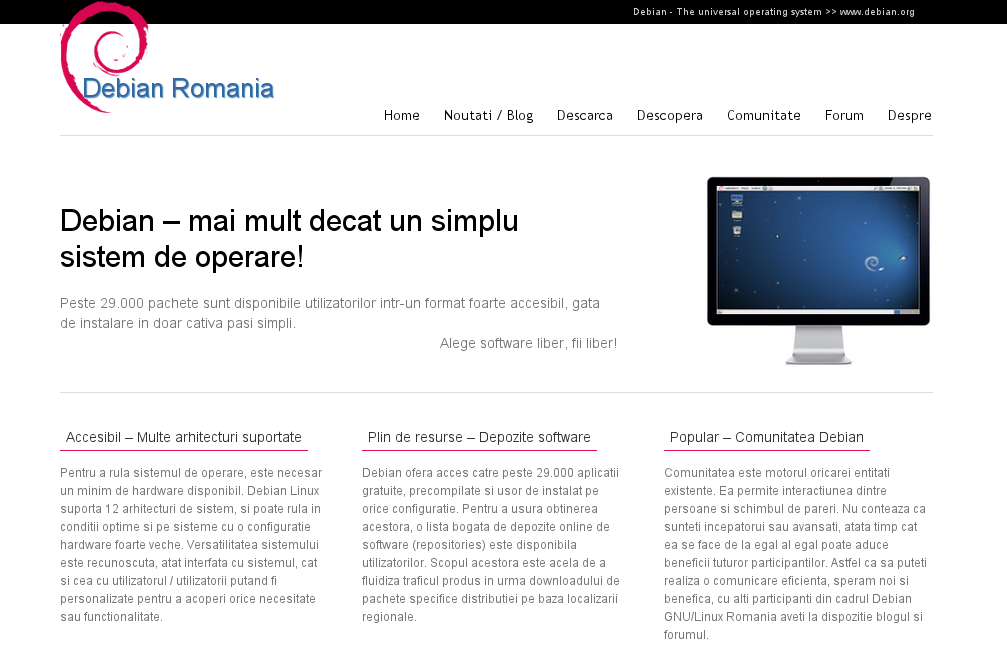
\includegraphics[height=2cm]{../images/dlro.png}
    \end{pgfpicture}
  }
\end{frame}

\begin{frame}
\frametitle{Povestea debian-linux.ro}
\begin{block}{}
...și va prinde forțe proaspete în iunie 2012!\\
\hfill\\
Ce vrem să facem:
\begin{itemize}
\item Un sit plin de resurse utile
\item Ghiduri, tutoriale, cursuri și ateliere
\item Traduceri și promovare
\end{itemize}
\end{block}
  \raisebox{0mm}[0mm][0pt]{%
    \begin{pgfpicture}{-80mm}{-17mm}{0mm}{0mm}
		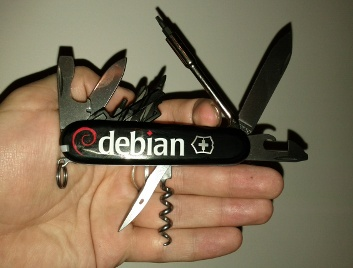
\includegraphics[height=2cm]{../images/debswiss.jpg}
    \end{pgfpicture}
  }
\end{frame}

\subsection{Proiecte și planuri}
\begin{frame}
\frametitle{Ce facem noi acum?}
\begin{itemize}
\item Traducerea manualului liber \emph{Debian Administrator's Handbook}, scris de Raphael Hertzog și Roland Mas
\item Planificăm situl debian-linux.ro în vederea transformării
\item Organizăm întâlniri!
\item Antrenăm comunitatea
\end{itemize}
\end{frame}

\begin{frame}
\frametitle{Ce putem face în continuare?}
\begin{itemize}
\item Atelier.deb (sau cum să împachetezi resurse pentru Debian)
\item Installfest
\item Ședințe tehnice (~MiniDebConf)
\item Întâlniri de eliminare a defectelor (Bug Squashing Party)
\item Petreceri de lansare (\emph{nu e greu, sunt rare} \smiley )
\end{itemize}
\end{frame}

\begin{frame}
\frametitle{Ce vrem să obținem?}
\begin{itemize}
\item Un număr crescut de contribuții 100\% românești
\item Mai mulți membri și dezvoltatori în cadrul Debian
\item Traducerea și publicarea regulată a DPN (en. \emph{Debian Project News})
\item O notorietate crescută a sistemului de operare în rândul utilizatorilor de GNU/Linux
\end{itemize}
\end{frame}


\section{Final} 
\begin{frame}
\centerline{Întrebări?}
\end{frame}
% End of slides
\end{document} 